

\section{Versuchsdurchführung}
\label{sec:Durchführung}
\subsection{Versuchsaufbau}
Der Versuchapparat, der auf dem Foto gezeigt wird, besteht aus zwei Pendeln mit verschiebbaren 
Pendelmassen der Masse $m=1kg$. Die effektive Länge der Pendel wird von der Aufhängung zum 
Mittelpunkt der Massen gemessen. Die Aufhängung besteht aus zwei spitzen in einer keilförmigen 
Nut, um Reibung zu minimieren. Weiterhin wird zur Bestimmung der Periodendauern eine Stoppuhr 
verwendet. Die Pendel werden mit einer Feder mit Kopplungsgrad K verbunden.
\begin{figure}
    \centering
    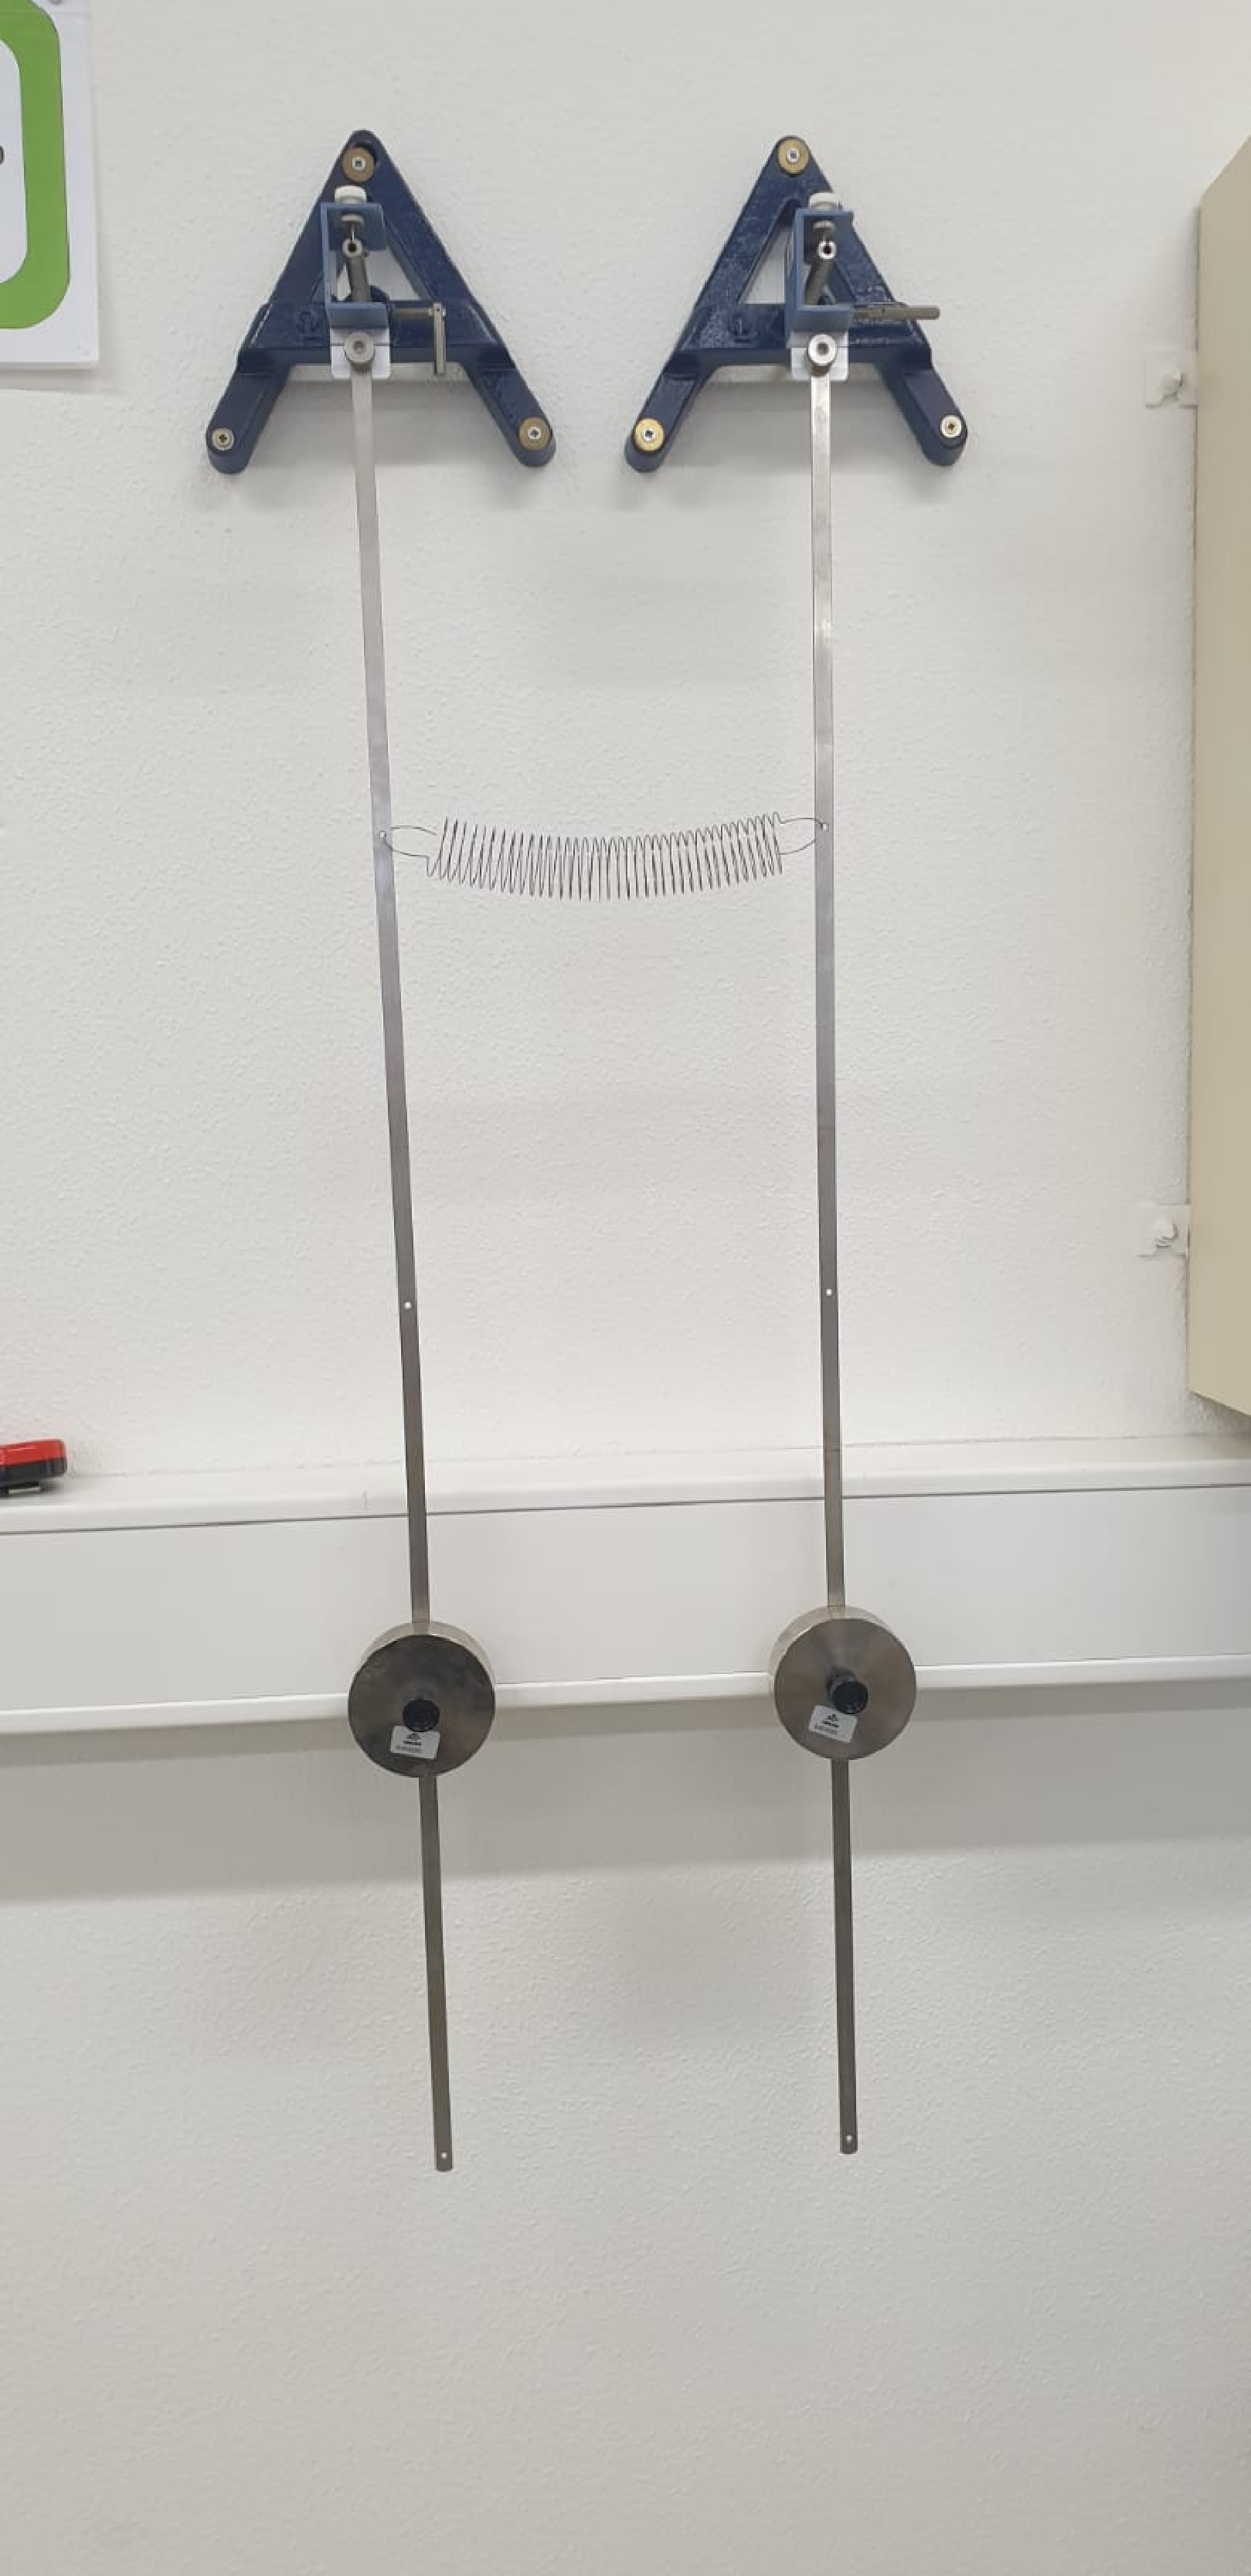
\includegraphics[width=9.71cm,height=20cm]{Bild.pdf}
    \caption{Versuchsaufbau}
    \label{fig:Versuchsaufbau}
  \end{figure}
\subsection{Durchführung}
Zunächst müssen die Pendel auf eine einheitliche Länge gebracht werden. 
Anschließend werden für beide Pendel jeweils einmal die Periodendauer gemessen 
und verglichen, um größere Abweichungen auszuschließen. Anschließend wurden zunächst 
für beide Pendel einzeln im ungekoppelten Zustand eine Messreihe zur Dauer der Eigenschwingung 
durchgeführt. Dies geschah indem die Pendel jeweils zehn mal ausgelenkt wurden, um mithilfe der 
Stoppuhr die Zeit zu messen, die das Pendel für fünf vollständige Schwingungen benötigt. Dadurch 
kann die Messabweichung der Periodendauer gering gehalten werden. \newline Anschließend wurden die 
Pendel durch die Feder verbunden und dem gleichen Schema folgend die Periodendauer der gleichsinnigen 
Schwingung $T_+$ gemessen.  \newline Danach wurde, ebenfalls in eine Reihe mit 10 Messungen, 
die Periodendauer der gegensinnigen Schwingung gemessen. Um zu gewährleisten, dass die Auslenkwinkel 
übereinstimmen wurden entsprechende Markierungen verwendet. \newline Zuletzt wurde eine gekoppelte 
Schwingung betrachtet. Dafür wurde zehnmal die Dauer für fünf Perioden eines der beiden Pendel bei 
anfänglichem Stillstand des anderen gemessen. Außerdem wurde zehn mal die Zeit gemessen die das Pendel, 
das sich zu Begin in Ruhe befindet, benötigt um wieder in Ruheposition zu gelangen, also die Dauer einer 
vollständigen Schwebung. Danach wurden die Pendel auf eine neue Länge justiert und alle zuvor beschriebenen 
Messreihen nach identischem Schema wiederholt. 
